
%(BEGIN_QUESTION)
% Copyright 2006, Tony R. Kuphaldt, released under the Creative Commons Attribution License (v 1.0)
% This means you may do almost anything with this work of mine, so long as you give me proper credit

An oil sump for a hydraulic system is equipped with a float-type level switch for sensing low oil level and providing automatic shut-down capability for the hydraulic system:

$$\includegraphics[width=15.5cm]{i00298x01.eps}$$

The flow rate of oil through the sump is quite high, and this presents a problem.  With the oil being so turbulent, the float does not rest gently on the oil's surface.  Instead, it is tossed to and fro on the choppy surface, which can make the level switch ``think'' the float has gone down further than it actually has, thus causing needless shutdowns.

One solution to this problem is a {\it stilling well}.  Describe what a ``stilling well'' is, how you might make one for this application, and why it works to prevent the problem.

\vskip 20pt \vbox{\hrule \hbox{\strut \vrule{} {\bf Suggestions for Socratic discussion} \vrule} \hrule}

\begin{itemize}
\item{} Would an ultrasonic level switch be immune to the turbulence?  Explain why or why not.
\end{itemize}

\underbar{file i00298}
%(END_QUESTION)





%(BEGIN_ANSWER)

I'll let you figure out the solution to this!

%(END_ANSWER)





%(BEGIN_NOTES)

A {\it stilling well} is a vertical pipe placed in the process liquid, designed to produce a calm (``still'') liquid surface for a level-sensing instrument to measure.  They are especially useful when sensing the level of a flowing stream of liquid, where anything placed within that flowing stream will be pushed laterally by the force of the moving liquid.

$$\includegraphics[width=15.5cm]{i00298x02.eps}$$

A simple piece of pipe works great as a stilling well.  One must take precautions that the float cannot get ``hung up'' inside the pipe, but otherwise the selection and installation of the pipe should be rather simple.

%INDEX% Switch, level: used with stilling well

%(END_NOTES)


